% This is samplepaper.tex, a sample chapter demonstrating the
% LLNCS macro package for Springer Computer Science proceedings;
% Version 2.20 of 2017/10/04
%
\documentclass[runningheads]{llncs}
%
\usepackage{graphicx}
\usepackage{subcaption}
\usepackage{float}
\usepackage{todonotes}
\usepackage{amsmath}
\usepackage{wrapfig}
% Used for displaying a sample figure. If possible, figure files should
% be included in EPS format.
%
% If you use the hyperref package, please uncomment the following line
% to display URLs in blue roman font according to Springer's eBook style:
% \renewcommand\UrlFont{\color{blue}\rmfamily}

\begin{document}
%
\title{Embedded Reachability for Half the Price\thanks{Supported by NSF Award 1925500.}}
%
%\titlerunning{Abbreviated paper title}
% If the paper title is too long for the running head, you can set
% an abbreviated paper title here
%
\author{Nathan Jewell\inst{1} \and
Stanley Bak\inst{2}\and
Houssam Abbas\inst{1}} 
%
\authorrunning{N. Jewell et al.}
% First names are abbreviated in the running head.
% If there are more than two authors, 'et al.' is used.
%
\institute{Oregon State University, Corvallis OR 97333, USA \and
Stony Brook University, Stony Brook NY, 11794, USA}
%
\maketitle              % typeset the header of the contribution
%
\begin{abstract}
Reachability analysis enables the safety assurance of control systems despite uncertain initial conditions and control inputs, and can be an important component to run on-board an autonomous system.
This tool paper demonstrates that it is possible to obtain accurate, real-time reachability computations for an autonomous vehicle using only simple kinematics, parallelization on a GPU without algorithmic changes, and while running a full autonomous racing stack.
%The tool we developed, QuickZono, is a variant of HYLAA, a state-of-the-art linear reachability tool.
%This stands in contrast to existing work which required the development of custom parallelizable reachability algorithms, the use of accurate nonlinear models of the dynamics, and was limited to a shorter look-ahead horizon. 
Our solution uses simple linearized kinematics, yet it is accurate; runs in Python, yet is real-time; shares the hardware with a full autonomous racing stack; and is partitioned between CPU and GPU using only code-level parallelization.
Thus this work lowers the barrier to running reachability significantly.
In our testing we achieve accurate 10-step reachability as quickly as 150 milliseconds. 
We also find that porting portions of reachability onto the GPU can improve the runtime for 10-step reachability by 62\% over a CPU-only implementation.
We demonstrate our results on the F1/10 1/10th-scale autonomous race car.
\keywords{Reachability  \and Safety Analysis \and CUDA \and GPU}
\end{abstract}
%
%
%
\section{Introduction}
For dynamical systems, \textit{reachability analysis} is the computation of possible future system states, given a \textit{set} of initial states and a \textit{set} of possible inputs at each time step. 
In discrete-time reachability, a range of $N$ reach sets are computed for $N$ future times $dt$, $2dt$,..., $Ndt$, with the guarantee that any state actually reached at time $i\cdot dt$ is within the $i^{th}$ computed reach set; thus the latter can be utilized for safety analysis \cite{malerintro}.
Specifically, with safety-critical systems, it is necessary to verify that no error state could be reached. In autonomous vehicles, error states may involve intersections with walls, other cars or people, etc.. By checking that the reach set does not contain error states, a guarantee is obtained that the next $N$ time steps are safe.  
If not, planned inputs can then be modified to avoid danger, preventing potentially catastrophic system failure. 

We have two objectives in this work: first is to enable reachability analysis for ground vehicles \textit{early in the design cycle}, so reachability itself becomes a rigorous \textit{design tool} - i.e., it is used to modify the design to better separate reach sets from error states.
This requires the ability to run reachability with minimal up-front effort, in real-time.
Minimal effort means using a simple dynamical model, little to no system identification, and no algorithmic modifications. 
Our second objective is to equip the F1/10 autonomous racing platform with an easy-to-use reachability tool. 
F1/10 (see f1tenth.org) is an open-source hardware and software platform for autonomous systems research and education, in use in tens of universities in the US and around the world, and the F1/10 project hosts yearly autonomous races. 
To enable formal methods education, and to make the platform safer for research and racing, reachability is an essential component. 
Embedded reachability on-board F1/10 must run out-of-the-box. Because different groups will have slightly different builds of the car, we cannot require custom dynamical models and system identification.

In this work we developed QuickZono, a variant of HYLAA\cite{hylaa}, a state-of-the-art linear reachability tool.
We show empirically, via experiments on the F1/10 race car, that the computations are still accurate, and real-time. 

\paragraph{Related work}. GPU-based implementations of dynamical systems reachability include Xspeed which introduces algorithms optimized for GPU performance \cite{xspeed}. Xspeed modifies reachability algorithms to enable GPU parallelization, unlike our approach. Because we use simple linearized kinematics, we also achieve faster runtimes compared to what's reported in~\cite{xspeed}.
The work in \cite{althoff} does real-time reachability on a non-linear model which requires systems identification, which is a step we seek to avoid.
%We explore a number of different runtime modes for profiling reachability computation. These modes are chosen to stress different components of the host system, improve runtime, and demonstrate the impact of a functional autonomous navigation stack on performance.

\section{Background}
\subsection{F1/10 Platform}
Our experiments used the F1/10 autonomous race car, which is an open-source platform designed for research and education on high-reliability autonomous systems. The F1/10 vehicle consists of a modified one tenth-scale remote control car chassis and is equipped with an improved electronic speed controller and LIDAR. The compute platform is an embedded NVIDIA Jetson TX2 computer. The Jetson TX2 is equipped with a dual CPU setup providing 6 (4+2) physical cores as well as a 256-core NVIDIA GPU and 8GB RAM. F1/10 runs a combination of low-level nodes to interface with hardware, publicly available SLAM algorithms, and a state-of-the-art model predictive contour controller \cite{mpcc}. 
It also includes the reachability software described next.

\subsection{The HYLAA Tool and its QuickZono variant}
HYLAA \cite{hylaa} is a state-of-the-art linear reachability analysis tool - that is, it can handle linear hybrid dynamical systems.
HYLAA output is a collection of reach sets. %A reach set is a tight over-approximation of all possible \emph{reachable} states at some future time $t$ (it is known to be theoretically impossible to obtain an exact representation of a reach set except in very special cases). 
%HYLAA adopts a simulation-equivalent approach where the linear superposition principle is applied to reduce the number of necessary simulations to $N+1$ for each simulated step in a N-dimensional system. 
Safety conditions are represented as unsafe polytopes in state-space that should be avoided (a polytope is a bounded intersection of half-spaces). 
The check of whether a reach set intersects an unsafe polytope reduces to a linear feasibility problem and is performed inline with the reachability analysis. 
%A variety of configuration options are provided to accommodate a variety of hybrid systems with changing dynamics.

\textbf{QuickZono: a HYLAA variant.}
QuickZono is a variant of HYLAA which we obtained by disabling certain unneeded features, and by GPU parallelization, as described in Section~\ref{sec:Parallelizing Reachability}. 
We did not modify the core HYLAA algorithms.
Many features of HYLAA were secondary to the task of generating the core set of reachable states.
Thus we disabled them.
%Instead of using the formalism of hybrid automata, QuickZono uses zonotopes to represent the agent state and perform the reachability simulation. 
%The agent state at time $t$, $S_t$ is used to compute the next reachable set $S_{t+dt}$ at time $t + dt$ where $dt$ is the discretization step-size. The computation is in the form $S_{t+dt} = S_t \cdot A + I_t \cdot B$ where $I_t$ is the planned inputs at time $t$ and matrices $A, B$ are the dynamics for the system. 
%In our experiments these dynamics are obtained by successive linearization as explained in the next section.
While the system state can be $n$ dimensional for any $n$, the unsafe sets for an autonomous vehicle are 2-dimensional obstacles in the $(x,y)$ plane. 
QuickZono still produces the  2-dimensional projections of reach sets onto $(x,y)$, necessary for checking the safety conditions.
QuickZono also defers the checking of safety conditions until after all reach sets are computed, rather than inline this check as in HYLAA.

\subsection{Successively Linearized Kinematics}

We use a simple 3 variable kinematic model for the car:
\begin{equation}
\dot{x} = v \cos{\psi + d},~\dot{y} = v \sin{\psi + d},~\dot{\psi} = v \frac{1}{L} \sin(d)
\end{equation}
where the state variable $\psi$ is the current yaw of the vehicle. The input variable $d$ is the steering angle in the vehicle's frame. The constant $L=.32$ is the wheel length of the vehicle in meters. 
Define the state vector, $S= [x, y, \psi]$, and the input vector  $U = [v, d]$.
An on-board Model Predictive Contouring Control  (MPCC) algorithm provides a sequence of optimal inputs for the next $N$ steps, $U_1,...,U_N$, and the corresponding predicted state trajectory is $S_1,...,S_N$. 
The non-linear kinematics are linearized around each $(S_t,U_t)$, thus obtaining the matrices $A_t,B_t$, and the linearized dynamics at step $t$ are then $S_{t+1} = S_t \cdot A_t + U_t \cdot B$.
A correction parameter $\alpha$ is introduced to scale the steering angle prior to evaluation of the Jacobian matrices 
$$\bar{S}_t = [\bar{x}, \bar{y}, \alpha\cdot\bar{\psi}]$$
This parameter was added to address the problem of over or under steering in the linearized kinematics and was tuned experimentally to $\alpha=.5$ 
See Fig.~\ref{fig:correctness}.


\begin{wrapfigure}{R}{.5\textwidth}
    \centering
    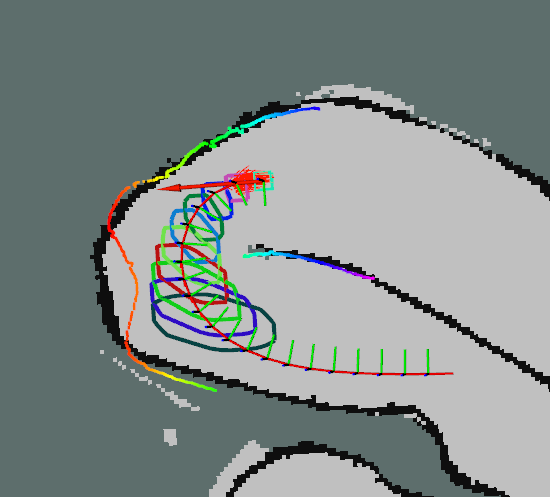
\includegraphics[width=.48\textwidth]{screenshots/FinalTopCorner.png}
    \caption{Zonotope projections from a 10-step reachability problem computed in realtime (multicolored polygons). Visualization is rendered in Rviz and shows the rasterized map in the background, overlayed by LIDAR scan data (multicolored points), MPCC trajectory (red line), and vehicle position/heading (red arrows). Note the MPCC trajectory lies inside the reach sets.}
    \label{fig:correctness}
\end{wrapfigure}

\section{Parallelizing Reachability}
\label{sec:Parallelizing Reachability}
Initial profiling of QuickZono using pycallgraph and cProfile revealed the large portion of computation time was spent projecting from n-dimensional zonotopes onto the useful 2-dimensional polygons which can be used to analyze safety parameters in the lower dimensional agent environment. So, this projection step was chosen as the most impactful target for parallelization. The projection was particularly well suited for this because it depends only on the target zonotope and thus is conceptually easy to parallelize across all $N$ output zonotopes.

GPU parallelization using CUDA was then written without modifying the underlying algorithm for the most time intensive function in QuickZono which is called recursively in the projection algorithm. The iterative CPU code was directly translated into a single CUDA Kernel ~\ref{fig:HybridComp}. While this section was the most time consuming piece of code, synchronous iteration was not completely avoided for the zonotope projection. Convex Hull computation was not moved to the GPU, resulting in additional copies between the host and the device to occur for each iteration of the synchronous loop. 
Effort was taken to minimize the number of memory copies to and from the GPU and compute resources were dynamically allocated depending on the number of vertices being considered in that particular convex hull as well as the dimension of the reachability problem. 
This implementation method of rewriting the code directly as one CUDA kernel abuses GPU thread abstractions to simplify translation. 
However, CUDA blocks (of threads) suffer from a constrained scalability compared to CUDA grids (of blocks) due to the memory layout on Nvidia GPUs ~\cite{cuda}. 
So, while we used shared memory to speed communication between threads within each block we also sacrificed the parallelism afforded by much larger grid sizes in this implementation.

\begin{figure}[t]
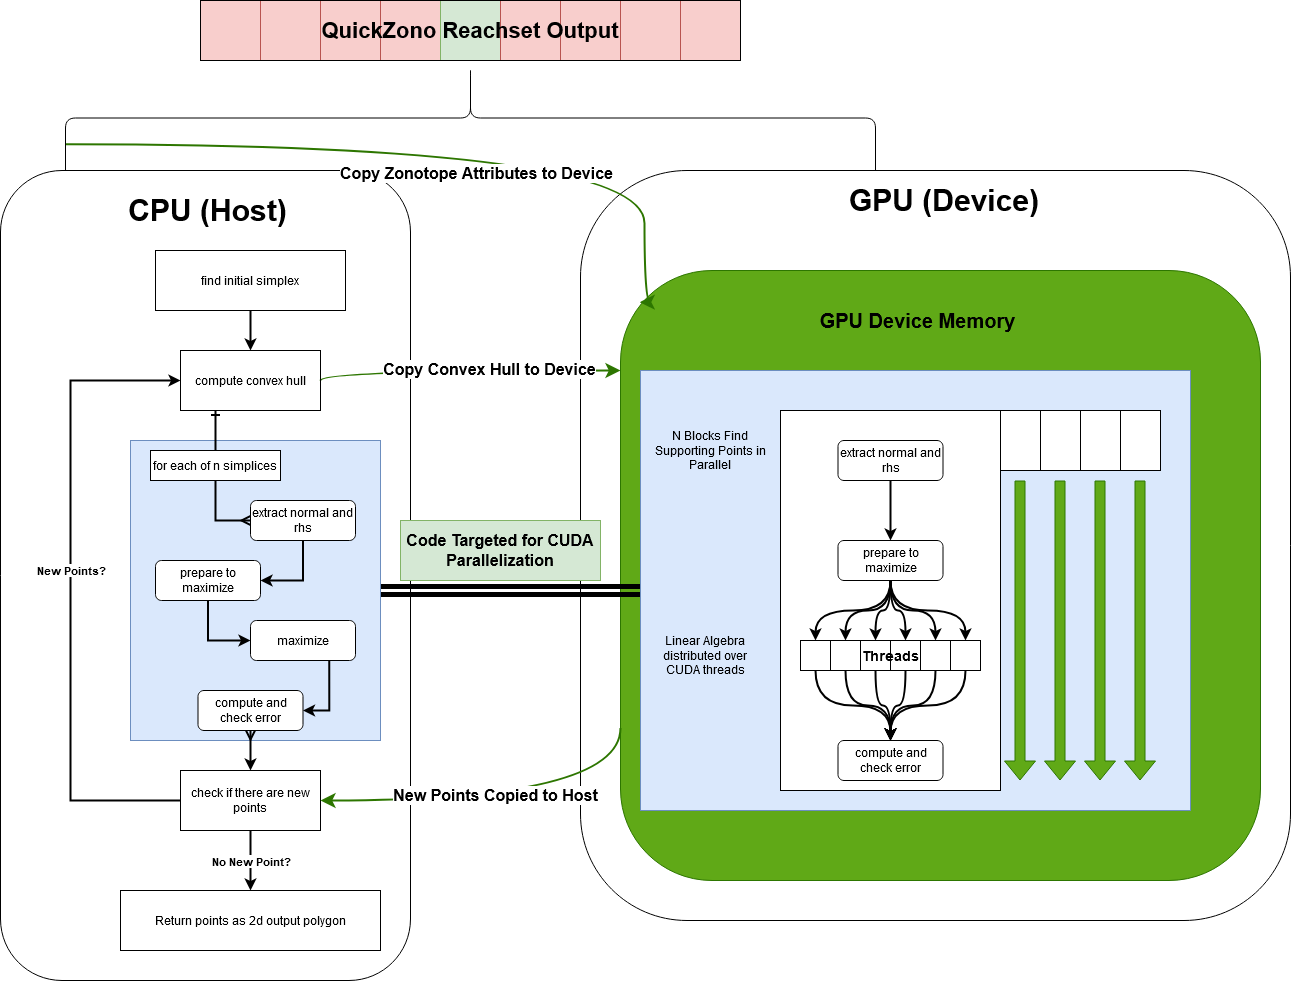
\includegraphics[width=\textwidth]{QZ_HYBRID_COMPUTATION.png}
\caption{The QZ\_HYBRID runtime mode implements a CPU/GPU hybrid computation model. Synchronous nested loops are translated to asynchronous grids of CUDA blocks in 2 dimensions. Matrix functions are distributed across 3 dimensions of threads within each block. The light blue blocks on the host and device perform analogous computations but, when executed on the GPU, as in QZ\_HYBRID, the work is distributed across hundreds of worker threads.} \label{fig:HybridComp}
\end{figure}
\section{Experimental Setup}


\subsection{Runtime Modes}
We compare three ways of distributing the code between the CPU cores and the GPU cores:

%\subsubsection{HYLAA} \newline The original hybrid reachability tool [cite].
%\vspace*{-10pt}
\textbf{Quickzono Single Core} [QZ\_CPU]: A simplified subset of HYLAA code with succinct wrappers. 

\textbf{Quickzono Multiple Core} [QZ\_MP]: Quickzono code with a trivial CPU-based multiprocessing model \newline applied to the projection step. 

\textbf{Quickzono GPU Hybrid} [QZ\_HYBRID]: Hybrid GPU/CPU implementation, with the most taxing part of the projection algorithm moved onto the GPU device. 


\subsection{Profiling Reachability Within the Stack}

In \textit{offline} profiling, reachability is computed as the sole program running on the system. 
In \textit{online} profiling, reachability is computed as part of a ROS network running physical control nodes (controller input, motor and servo control, etc.), a GPU-based particle filter node for localization, a model predictive control node, and various other supporting nodes. The MPCC is configured to use 15 time steps of .15 sec each, generating control inputs at a rate of about 20hz.
%Before beginning the profiling, the vehicle is placed into the test track, localized and configured to autonomously drive the track until profiling is complete. 
%The reachability node is implemented as a wrapper for the various reachability modes described above and records call timings for the same function, executing as quickly as possible. 

\paragraph{Performance Characteristics}
Evaluating an embedded reachability algorithm is done using the following metrics: 
1) first of course is correctness: namely that the computed set is indeed a reachset for the dynamics. To validate correctness, we used HYLAA output as the ground truth.
%
2) Next is runtime: running a safety algorithm is only effective when there is a low latency between consecutive executions. Otherwise, safety analysis results could be too late for the agent to develop a response. 
A dedicated testing script executes each of the runtime modes for 200 trials, for $N$ reachability steps where $N$ is between 4 and 24. 
We report average and standard deviation of runtimes over the 200 trials.
%HYLAA is only tested over 5 trials due to slow performance. 
The script outputs timing data excluding any one-off setup and configuration code.
%
3) Third is scalability with the number $N$ of reachability time steps. 
%
4) Finally is runtime variability: The consistency of the tool's runtime is paramount for autonomous systems.
Runtime spikes at the wrong time could create dangerous situations for the agent. 
Runtime variability is measured by runtime standard deviation, and we also report the  95\% confidence intervals around the mean assuming normally distributed variation in runtimes.


\section{Results}

\begin{figure}[t]
\centering
\begin{minipage}{.5\textwidth}
    \centering
    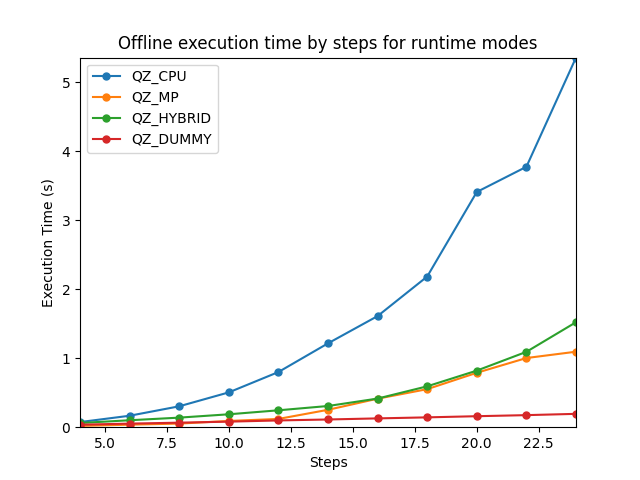
\includegraphics[width=\linewidth]{profiler_out/offline_avg_unified.png}
    \caption{Average Offline trial execution times for all runtime modes.} \label{fig:offline_avg}
\end{minipage}%
\begin{minipage}{.5\textwidth}
    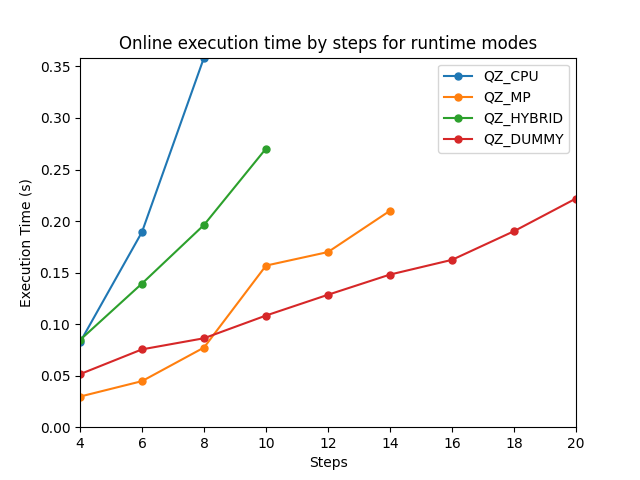
\includegraphics[width=\linewidth]{profiler_out/online_avg_unified.png}
    \caption{Average Online trial execution times for all runtime modes.} \label{fig:online_avg}
\end{minipage}
\end{figure}
\begin{wrapfigure}{L}{.5\textwidth}
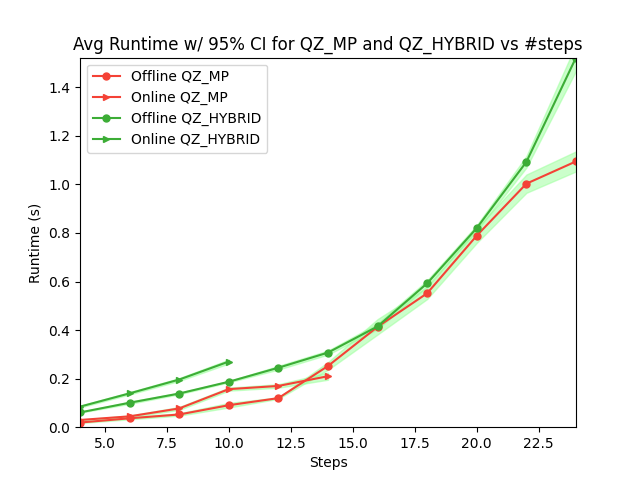
\includegraphics[width=.48\textwidth]{profiler_out/avg_mp_hybrid_CI.png}
\caption{Comparison between Multiprocessing and Hybridized online and offline runtimes.} \label{fig:mp_hybrid_ci}
\end{wrapfigure}

Realtime reachability performance at 4hz or greater was achieved for both QZ\_MP and QZ\_HYBRID runtime modes. This represents a significant performance improvement over QZ\_CPU for both methods of parallelization ( Fig. ~\ref{fig:correctness}). We achieved an improvement in runtime based on straightforward techniques for GPU Parallelization with Nvidia CUDA. This is important because GPU resources are more powerful than CPU resources if they can be properly utilized. Process based parallelization on in QZ\_MP showed improvement larger than \%60 at 10 time steps over QZ\_CPU. But the multiprocessing attempt strained four CPU cores which may be better utilized in other critical applications. Notably, 

Online modes had generally higher runtimes (slower) than offline modes for all steps across all rutnime modes. This is sensible due to increased CPU load in online mode from SLAM + MPCC algorithms (Fig. ~\ref{fig:online_avg}) Despite improved scalability of QZ\_HYBRID vs QZ\_CPU (Fig. ~\ref{fig:offline_avg}) the two runtime modes have comparable timings at the lowest number of reachability steps. The overhead of making CUDA device calls for initializing GPU memory in QZ\_HYBRID may explain this discrepancy.

Comparison of QZ\_MP and QZ\_HYBRID shows a much larger 95\% confidence interval for CPU\_MP  in the offline mode. This is unexpected given anticipated variation introduced by calling CUDA functions (Fig. ~\ref{fig:mp_hybrid_ci}). While online execution of QZ\_HYBRID is slower than QZ\_MP, offline timings are very similar for the two modes between 14 and 22 steps. So, performance of QZ\_HYBRID is comparable to that of QZ\_MP at these configurations despite only utilizing a single CPU core. This indicates a potential for reduced CPU load without sacrificing reachability performance through only naive parallelization techniques.


%
% ---- Bibliography ----
%
% BibTeX users should specify bibliography style 'splncs04'.
% References will then be sorted and formatted in the correct style.
%
\bibliographystyle{splncs04}
\bibliography{bibliography}
%
%
\end{document}
